\documentclass[tikz,10pt,border=.1mm]{standalone}
\usepackage{amsmath,amsfonts,amssymb,siunitx,float,subcaption,setspace,booktabs,diagbox,bm,tikz,structmech,mathtools,tikz-3dplot,pgfplots,url}
\usetikzlibrary{decorations.pathmorphing,shapes.geometric,spy}
\pgfplotsset{compat=1.18}
\newcommand{\balpha}{\mb{\alpha}}
\newcommand{\bbeta}{\mb{\beta}}
\newcommand{\bc}{\mb{c}}
\newcommand{\bd}{\mb{d}}
\newcommand{\be}{\mb{e}}
\newcommand{\beeta}{\mb{\eta}}
\newcommand{\bgamma}{\mb{\gamma}}
\newcommand{\bn}{\mb{n}}
\newcommand{\bq}{\mb{q}}
\newcommand{\bs}{\mb{s}}
\newcommand{\bsigma}{\mb{\sigma}}
\newcommand{\bv}{\mb{v}}
\newcommand{\bvarepsilon}{\mb{\varepsilon}}
\newcommand*{\algoref}[1]{Algorithm~\ref{#1}}
\newcommand*{\ddfrac}[2]{\dfrac{\md{#1}}{\md{#2}}}
\newcommand*{\dev}[1]{\text{dev}\left(#1\right)}
\newcommand*{\diag}[1]{\text{diag}\left(#1\right)}
\newcommand*{\eqsref}[1]{Eq.~(\ref{#1})}
\newcommand*{\figref}[1]{Fig.~\ref{#1}}
\newcommand*{\mb}[1]{\bm{#1}}
\newcommand*{\md}[1]{\mathrm{d}#1}
\newcommand*{\mT}{\mathrm{T}}
\newcommand*{\pdfrac}[2]{\dfrac{\partial{#1}}{\partial{#2}}}
\newcommand*{\sign}[1]{\text{sign}\left(#1\right)}
\newcommand*{\tabref}[1]{Table~\ref{#1}}
\newcommand*{\tr}[1]{\text{trace}\left(#1\right)}
\definecolor{d73027}{HTML}{d73027}
\definecolor{fc8d59}{HTML}{fc8d59}
\definecolor{fee090}{HTML}{fee090}
\definecolor{e0f3f8}{HTML}{e0f3f8}
\definecolor{91bfdb}{HTML}{91bfdb}
\definecolor{4575b4}{HTML}{4575b4}
\begin{filecontents}{tmp/cot.txt}
    1.000000000000000072e-17 1.000000000000000072e-17
    1.000000000000000102e-16 1.000000000000000965e-16
    1.000000000000000078e-15 1.000000000000001853e-15
    1.000000000000000157e-14 1.000000000000020194e-14
    1.000000000000000157e-13 1.000000000000200212e-13
    1.000000000000000182e-12 1.000000000001999875e-12
    1.000000000000000101e-11 1.000000000020000100e-11
    1.000000000000000166e-10 1.000000000200000159e-10
    1.000000000000000269e-09 1.000000001999999740e-09
    1.000000000000000352e-08 1.000000020000000027e-08
    1.000000000000000352e-07 1.000000199999953167e-07
    1.000000000000000378e-06 1.000001999995333917e-06
    1.000000000000000421e-05 1.000019999533329526e-05
    1.000000000000000454e-04 1.000199953329336327e-04
    1.000000000000000454e-03 1.001995329357778129e-03
    1.000000000000000541e-02 1.019529575707463567e-02
    1.000000000000000611e-01 1.151480769627777345e-01
    1.000000000000000666e+00 3.385055658903006748e-01
    1.000000000000000711e+01 4.630732723445631083e-02
    1.000000000000000711e+02 4.418060505895468441e-03
\end{filecontents}
\begin{filecontents}{tmp/log.txt}
    1.000000000000000072e-17 2.618186755244390762e-02
    1.000000000000000102e-16 2.785911581279704521e-02
    1.000000000000000078e-15 2.976560548684022145e-02
    1.000000000000000157e-14 3.195169429583541443e-02
    1.000000000000000157e-13 3.448362391126010701e-02
    1.000000000000000182e-12 3.745030384096753595e-02
    1.000000000000000101e-11 4.097388726142127402e-02
    1.000000000000000166e-10 4.522685763844839363e-02
    1.000000000000000269e-09 5.046081844034946973e-02
    1.000000000000000352e-08 5.705749577733557759e-02
    1.000000000000000352e-07 6.562476851935679367e-02
    1.000000000000000378e-06 7.719169042942151948e-02
    1.000000000000000421e-05 9.364470919725104148e-02
    1.000000000000000454e-04 1.188362575230943047e-01
    1.000000000000000454e-03 1.619459754153584619e-01
    1.000000000000000541e-02 2.506407737562225679e-01
    1.000000000000000611e-01 4.984985479103578032e-01
    1.000000000000000666e+00 6.661338147750942201e-16
    1.000000000000000711e+01 2.411291696523686079e-01
    1.000000000000000711e+02 1.648229424204348259e-01
\end{filecontents}
\begin{filecontents}{tmp/pow1.txt}
    1.000000000000000072e-17 3.162277675168379692e-09
    1.000000000000000102e-16 1.000000014999999943e-08
    1.000000000000000078e-15 3.162277810168368486e-08
    1.000000000000000157e-14 1.000000149999967544e-07
    1.000000000000000157e-13 3.162279160167351782e-07
    1.000000000000000182e-12 1.000001499996749825e-06
    1.000000000000000101e-11 3.162292660065604651e-06
    1.000000000000000166e-10 1.000014999674998486e-05
    1.000000000000000269e-09 3.162427649890790397e-05
    1.000000000000000352e-08 1.000149967498126599e-04
    1.000000000000000352e-07 3.163776632241084553e-04
    1.000000000000000378e-06 1.001496748139050867e-03
    1.000000000000000421e-05 3.177174703079323984e-03
    1.000000000000000454e-04 1.014673264388731531e-02
    1.000000000000000454e-03 3.301855901292539974e-02
    1.000000000000000541e-02 1.116877974792942763e-01
    1.000000000000000611e-01 3.725995555786141278e-01
    1.000000000000000666e+00 7.298437881283574846e-01
    1.000000000000000711e+01 5.386782170348952681e-01
    1.000000000000000711e+02 4.524857753640627034e-01
\end{filecontents}
\begin{filecontents}{tmp/pow2.txt}
    1.000000000000000072e-17 1.000000000000000072e-17
    1.000000000000000102e-16 1.000000000000000965e-16
    1.000000000000000078e-15 1.000000000000001853e-15
    1.000000000000000157e-14 1.000000000000020194e-14
    1.000000000000000157e-13 1.000000000000200212e-13
    1.000000000000000182e-12 1.000000000001999875e-12
    1.000000000000000101e-11 1.000000000020000100e-11
    1.000000000000000166e-10 1.000000000200000159e-10
    1.000000000000000269e-09 1.000000001999999740e-09
    1.000000000000000352e-08 1.000000020000000027e-08
    1.000000000000000352e-07 1.000000199999949991e-07
    1.000000000000000378e-06 1.000001999995000398e-06
    1.000000000000000421e-05 1.000019999499994713e-05
    1.000000000000000454e-04 1.000199949994003693e-04
    1.000000000000000454e-03 1.001994994031992544e-03
    1.000000000000000541e-02 1.019494319012576034e-02
    1.000000000000000611e-01 1.146968336198978533e-01
    1.000000000000000666e+00 5.657414540893350718e-01
    1.000000000000000711e+01 4.074169802195639623e-01
    1.000000000000000711e+02 3.845270415093802185e-01
\end{filecontents}
\begin{filecontents}{tmp/pow3.txt}
    1.000000000000000072e-17 3.982972037698159469e-04
    1.000000000000000102e-16 6.314344601016684067e-04
    1.000000000000000078e-15 1.001197559479824343e-03
    1.000000000000000157e-14 1.587897739110697131e-03
    1.000000000000000157e-13 2.519419228010421046e-03
    1.000000000000000182e-12 3.999936345421495169e-03
    1.000000000000000101e-11 6.356732645903701538e-03
    1.000000000000000166e-10 1.011755549399330836e-02
    1.000000000000000269e-09 1.614061885079053765e-02
    1.000000000000000352e-08 2.583720746837320226e-02
    1.000000000000000352e-07 4.155805366067209794e-02
    1.000000000000000378e-06 6.725895844505053178e-02
    1.000000000000000421e-05 1.095753646364497347e-01
    1.000000000000000454e-04 1.792048614575600385e-01
    1.000000000000000454e-03 2.914136611789981957e-01
    1.000000000000000541e-02 4.619783836552983081e-01
    1.000000000000000611e-01 6.918917370282156032e-01
    1.000000000000000666e+00 8.739448295698315494e-01
    1.000000000000000711e+01 7.341964831520501056e-01
    1.000000000000000711e+02 6.085974682202813790e-01
\end{filecontents}
\begin{filecontents}{tmp/pow4.txt}
    1.000000000000000072e-17 1.000000000000000141e-34
    1.000000000000000102e-16 1.000000000000000193e-32
    1.000000000000000078e-15 1.000000000000000083e-30
    1.000000000000000157e-14 1.000000000000000308e-28
    1.000000000000000157e-13 1.000000000000000325e-26
    1.000000000000000182e-12 1.000000000000000475e-24
    1.000000000000000101e-11 1.000000000000000166e-22
    1.000000000000000166e-10 1.000000000000000397e-20
    1.000000000000000269e-09 1.000000000000000457e-18
    1.000000000000000352e-08 1.000000000000000842e-16
    1.000000000000000352e-07 1.000000000000030291e-14
    1.000000000000000378e-06 1.000000000003000327e-12
    1.000000000000000421e-05 1.000000000300000738e-10
    1.000000000000000454e-04 1.000000030000000030e-08
    1.000000000000000454e-03 1.000002999990001025e-06
    1.000000000000000541e-02 1.000299899976012726e-04
    1.000000000000000611e-01 1.028977180887020657e-02
    1.000000000000000666e+00 3.819660112501050975e-01
    1.000000000000000711e+01 2.979207332185368484e-01
    1.000000000000000711e+02 2.967543918766996081e-01
\end{filecontents}
\begin{filecontents}{tmp/hardening.inverse.txt}
    0.000000000000000000e+00 0.000000000000000000e+00
    1.000000000000000056e-01 9.517818622144433305e-02
    2.000000000000000111e-01 1.813990350202696333e-01
    3.000000000000000444e-01 2.595835658904977472e-01
    4.000000000000000222e-01 3.305371390792684050e-01
    5.000000000000000000e-01 3.949984134600889041e-01
    6.000000000000000888e-01 4.536396756497711458e-01
    7.000000000000000666e-01 5.070668400084317184e-01
    8.000000000000000444e-01 5.558293277987650383e-01
    9.000000000000000222e-01 6.003884612604569737e-01
    1.000000000000000000e+00 6.411347473864134061e-01
    1.100000000000000089e+00 6.784330779308410664e-01
    1.200000000000000178e+00 7.126230180583709162e-01
    1.300000000000000044e+00 7.440188063440582589e-01
    1.400000000000000133e+00 7.729093547733824066e-01
    1.500000000000000000e+00 7.995582487422470130e-01
    1.600000000000000089e+00 8.242037366895583750e-01
    1.700000000000000178e+00 8.470368738693998534e-01
    1.800000000000000044e+00 8.682094750487496793e-01
    1.900000000000000133e+00 8.878649100594313559e-01
    2.000000000000000000e+00 9.061391544007555421e-01
    2.100000000000000089e+00 9.231607892395210513e-01
    2.200000000000000178e+00 9.390510014100141856e-01
    2.300000000000000266e+00 9.539235834140086245e-01
    2.400000000000000355e+00 9.678849334207662025e-01
    2.500000000000000000e+00 9.810340552670360204e-01
    2.600000000000000089e+00 9.934621252504135525e-01
    2.700000000000000178e+00 1.005237674690885541e+00
    2.800000000000000266e+00 1.016407432149403656e+00
    2.900000000000000355e+00 1.027015815873632443e+00
    3.000000000000000000e+00 1.037105839034464516e+00
    3.100000000000000089e+00 1.046719109726020447e+00
    3.200000000000000178e+00 1.055895830965649207e+00
    3.300000000000000266e+00 1.064674800693928169e+00
    3.400000000000000355e+00 1.073093411774662442e+00
    3.500000000000000000e+00 1.081187651994885757e+00
    3.600000000000000089e+00 1.088992104064859578e+00
    3.700000000000000178e+00 1.096539945618073997e+00
    3.800000000000000266e+00 1.103862949211246836e+00
    3.900000000000000355e+00 1.110990767115421551e+00
    4.000000000000000000e+00 1.117937788527934240e+00
    4.100000000000000533e+00 1.124712279241497193e+00
    4.200000000000000178e+00 1.131323820779194689e+00
    4.299999999999999822e+00 1.137781984283245729e+00
    4.400000000000000355e+00 1.144096330515004034e+00
    4.500000000000000000e+00 1.150276409854957604e+00
    4.600000000000000533e+00 1.156331762302730048e+00
    4.700000000000000178e+00 1.162271917477079031e+00
    4.800000000000000711e+00 1.168106394615896715e+00
    4.900000000000000355e+00 1.173844702576210874e+00
    5.000000000000000000e+00 1.179496339834183338e+00
    5.100000000000000533e+00 1.185070794485110657e+00
    5.200000000000000178e+00 1.190577544243424546e+00
    5.300000000000000711e+00 1.196026056442690999e+00
    5.400000000000000355e+00 1.201425788035611175e+00
    5.500000000000000000e+00 1.206786185594020289e+00
    5.600000000000000533e+00 1.212113906208689862e+00
    5.700000000000000178e+00 1.217405526554930839e+00
    5.800000000000000711e+00 1.222661329750559078e+00
    5.900000000000000355e+00 1.227882196197205733e+00
    6.000000000000000000e+00 1.233069113756864343e+00
    6.100000000000000533e+00 1.238223177751890614e+00
    6.200000000000000178e+00 1.243345590965002190e+00
    6.300000000000000711e+00 1.248437663639278883e+00
    6.400000000000000355e+00 1.253500813478162224e+00
    6.500000000000000000e+00 1.258536565645456129e+00
    6.600000000000000533e+00 1.263546552765326902e+00
    6.700000000000000178e+00 1.268532514922302568e+00
    6.800000000000000711e+00 1.273496299661272868e+00
    6.900000000000000355e+00 1.278439861987490600e+00
    7.000000000000000000e+00 1.283365264366569614e+00
    7.100000000000000533e+00 1.288274676724486367e+00
    7.200000000000000178e+00 1.293170376447579706e+00
    7.300000000000000711e+00 1.298054748382549750e+00
    7.400000000000000355e+00 1.302930284836459229e+00
    7.500000000000000000e+00 1.307799585576732815e+00
    7.600000000000000533e+00 1.312665357831157564e+00
    7.700000000000000178e+00 1.317530416287882256e+00
    7.800000000000000711e+00 1.322396478992998503e+00
    7.900000000000000355e+00 1.327257374445248939e+00
    8.000000000000000000e+00 1.332111903123012864e+00
    8.099999999999999645e+00 1.336960270394595751e+00
    8.200000000000001066e+00 1.341802691333118469e+00
    8.300000000000000711e+00 1.346639390716517726e+00
    8.400000000000000355e+00 1.351470603027545847e+00
    8.500000000000000000e+00 1.356296572453770777e+00
    8.599999999999999645e+00 1.361117552887576077e+00
    8.700000000000001066e+00 1.365933807926161592e+00
    8.800000000000000711e+00 1.370745610871542342e+00
    8.900000000000000355e+00 1.375553244730548963e+00
    9.000000000000000000e+00 1.380357002214828377e+00
    9.099999999999999645e+00 1.385157185740842456e+00
    9.200000000000001066e+00 1.389954107429869579e+00
    9.300000000000000711e+00 1.394748089108003075e+00
    9.400000000000000355e+00 1.399539462306152560e+00
    9.500000000000000000e+00 1.404328568260043042e+00
    9.600000000000001421e+00 1.409115757910215372e+00
    9.700000000000001066e+00 1.413901391902025795e+00
    9.800000000000000711e+00 1.418685840585646840e+00
    9.900000000000000355e+00 1.423469484016065989e+00
    1.000000000000000000e+01 1.428252711953087450e+00
\end{filecontents}
\begin{filecontents}{tmp/softening.inverse.txt}
    0.000000000000000000e+00 0.000000000000000000e+00
    1.000000000000000056e-01 9.514686290580821881e-02
    2.000000000000000111e-01 1.811639197857747297e-01
    3.000000000000000444e-01 2.588387998395766387e-01
    4.000000000000000222e-01 3.288738114420266534e-01
    5.000000000000000000e-01 3.919313457061204264e-01
    6.000000000000000888e-01 4.486341988760567112e-01
    7.000000000000000666e-01 4.995655723272378612e-01
    8.000000000000000444e-01 5.452742422764870200e-01
    9.000000000000000222e-01 5.862083929988679554e-01
    1.000000000000000000e+00 6.227553293287462211e-01
    1.100000000000000089e+00 6.552881198192859191e-01
    1.200000000000000178e+00 6.841656231346562311e-01
    1.300000000000000044e+00 7.097324880500309741e-01
    1.400000000000000133e+00 7.323191534515887113e-01
    1.500000000000000000e+00 7.522417305004924781e-01
    1.600000000000000089e+00 7.697699120219243518e-01
    1.700000000000000178e+00 7.850883012690428320e-01
    1.800000000000000044e+00 7.983678591513472256e-01
    1.900000000000000133e+00 8.097774288132130183e-01
    2.000000000000000000e+00 8.194837356338906531e-01
    2.100000000000000089e+00 8.276513872275067518e-01
    2.200000000000000178e+00 8.344428734430630046e-01
    2.300000000000000266e+00 8.400185663644369471e-01
    2.400000000000000355e+00 8.445365301647669298e-01
    2.500000000000000000e+00 8.481155202822235895e-01
    2.600000000000000089e+00 8.508138453231384180e-01
    2.700000000000000178e+00 8.526896942203314733e-01
    2.800000000000000266e+00 8.538035928991806189e-01
    2.900000000000000355e+00 8.542184042776214126e-01
    3.000000000000000000e+00 8.539993282661473284e-01
    3.100000000000000089e+00 8.532139017678096460e-01
    3.200000000000000178e+00 8.519319986782173393e-01
    3.300000000000000266e+00 8.502258298855372987e-01
    3.400000000000000355e+00 8.481699432704941088e-01
    3.500000000000000000e+00 8.458242451202764300e-01
    3.600000000000000089e+00 8.431938604474122911e-01
    3.700000000000000178e+00 8.402874850099493198e-01
    3.800000000000000266e+00 8.371173226477804930e-01
    3.900000000000000355e+00 8.336985313328798552e-01
    4.000000000000000000e+00 8.300492231693035183e-01
    4.100000000000000533e+00 8.261904643931888836e-01
    4.200000000000000178e+00 8.221462753727550865e-01
    4.299999999999999822e+00 8.179436306083026631e-01
    4.400000000000000355e+00 8.136124587322137724e-01
    4.500000000000000000e+00 8.091856425089525295e-01
    4.600000000000000533e+00 8.046989985048502714e-01
    4.700000000000000178e+00 8.001649739710200437e-01
    4.800000000000000711e+00 7.955682245008546261e-01
    4.900000000000000355e+00 7.909034034731651230e-01
    5.000000000000000000e+00 7.861674264439083570e-01
    5.100000000000000533e+00 7.813594711461870901e-01
    5.200000000000000178e+00 7.764809774902500239e-01
    5.300000000000000711e+00 7.715356475634920219e-01
    5.400000000000000355e+00 7.665294456304535542e-01
    5.500000000000000000e+00 7.614705981328212525e-01
    5.600000000000000533e+00 7.563695936894275773e-01
    5.700000000000000178e+00 7.512391830962510397e-01
    5.800000000000000711e+00 7.460943793264159796e-01
    5.900000000000000355e+00 7.409524575301926763e-01
    6.000000000000000000e+00 7.358315819950137504e-01
    6.100000000000000533e+00 7.307212247151037010e-01
    6.200000000000000178e+00 7.256073538938744294e-01
    6.300000000000000711e+00 7.204831537294514865e-01
    6.400000000000000355e+00 7.153432096498710813e-01
    6.500000000000000000e+00 7.101835083130796367e-01
    6.600000000000000533e+00 7.050014376069342337e-01
    6.700000000000000178e+00 6.997957866492023893e-01
    6.800000000000000711e+00 6.945667457875621675e-01
    6.900000000000000355e+00 6.893159065996021795e-01
    7.000000000000000000e+00 6.840462618928214722e-01
    7.100000000000000533e+00 6.787622057046294177e-01
    7.200000000000000178e+00 6.734695333023461572e-01
    7.300000000000000711e+00 6.681754411832021567e-01
    7.400000000000000355e+00 6.628885270743384295e-01
    7.500000000000000000e+00 6.576187899328066466e-01
    7.600000000000000533e+00 6.523776299455685823e-01
    7.700000000000000178e+00 6.471682994759047070e-01
    7.800000000000000711e+00 6.419778535000664199e-01
    7.900000000000000355e+00 6.367959032169486777e-01
    8.000000000000000000e+00 6.316135328605804178e-01
    8.099999999999999645e+00 6.264232990462125228e-01
    8.200000000000001066e+00 6.212192307703177097e-01
    8.300000000000000711e+00 6.159968294105909736e-01
    8.400000000000000355e+00 6.107530687259489222e-01
    8.500000000000000000e+00 6.054863948565302190e-01
    8.599999999999999645e+00 6.001967263236955841e-01
    8.700000000000001066e+00 5.948854540300275717e-01
    8.800000000000000711e+00 5.895554412593306814e-01
    8.900000000000000355e+00 5.842110236766314690e-01
    9.000000000000000000e+00 5.788580093281783245e-01
    9.099999999999999645e+00 5.735036786414415833e-01
    9.200000000000001066e+00 5.681567844251136368e-01
    9.300000000000000711e+00 5.628275518691087109e-01
    9.400000000000000355e+00 5.575276785445630878e-01
    9.500000000000000000e+00 5.522703344038348838e-01
    9.600000000000001421e+00 5.470614417786429096e-01
    9.700000000000001066e+00 5.418523088127243925e-01
    9.800000000000000711e+00 5.366340074365543167e-01
    9.900000000000000355e+00 5.314079876433578375e-01
    1.000000000000000000e+01 5.261756114902511605e-01
\end{filecontents}
\begin{filecontents}{tmp/conventional.criterion.txt}
    0.0000000000000000e+00   0.0000000000000000e+00   0.0000000000000000e+00   0.0000000000000000e+00   0.0000000000000000e+00   0.0000000000000000e+00
    1.4000000000000001e-01   8.0000000000000000e+00   1.8794895169376498e-04   1.4511420151610863e-01   0.0000000000000000e+00   3.0808187698990179e-02
    2.8000000000000003e-01   6.0000000000000000e+00   3.8733644114432155e-04   2.5431368763607815e-01   0.0000000000000000e+00   6.1969447413846274e-02
    4.2000000000000004e-01   5.0000000000000000e+00   5.9317003369944120e-04   3.4252629587639410e-01   0.0000000000000000e+00   9.2594080853256946e-02
    5.6000000000000005e-01   5.0000000000000000e+00   8.0369925723188743e-04   4.1632090708418162e-01   0.0000000000000000e+00   1.2238125421990988e-01
    7.0000000000000007e-01   5.0000000000000000e+00   1.0181269569735840e-03   4.7938432183554824e-01   0.0000000000000000e+00   1.5120602401126804e-01
    8.4000000000000008e-01   5.0000000000000000e+00   1.2360291295194041e-03   5.3405632309708806e-01   0.0000000000000000e+00   1.7901362670304766e-01
    9.8000000000000009e-01   5.0000000000000000e+00   1.4571486525575333e-03   5.8194078072319577e-01   0.0000000000000000e+00   2.0578195865488552e-01
    1.1200000000000001e+00   5.0000000000000000e+00   1.4571486525575333e-03   2.4743203742860501e-01   0.0000000000000000e+00   2.0578195865488552e-01
    1.2600000000000002e+00   5.0000000000000000e+00   1.4571486525575333e-03   1.4548819634045940e-01   0.0000000000000000e+00   2.0578195865488552e-01
    1.4000000000000004e+00   6.0000000000000000e+00   1.6264479557158101e-03   2.4166416790087894e-01   0.0000000000000000e+00   1.6971514080791264e-01
    1.5400000000000005e+00   5.0000000000000000e+00   1.8069234619642821e-03   3.2320150662060443e-01   0.0000000000000000e+00   1.3289510523627635e-01
    1.6800000000000006e+00   5.0000000000000000e+00   1.9960957503111173e-03   3.9373145709391755e-01   0.0000000000000000e+00   9.6009948103472964e-02
    1.8200000000000007e+00   5.0000000000000000e+00   2.1925190632060033e-03   4.5551296152805887e-01   0.0000000000000000e+00   5.9469088557853413e-02
    1.9600000000000009e+00   5.0000000000000000e+00   2.3952453855423795e-03   5.1009907587111247e-01   0.0000000000000000e+00   2.3539833509511495e-02
    2.0000000000000000e+00   5.0000000000000000e+00   2.4536747543090882e-03   5.2515205712214086e-01   0.0000000000000000e+00   1.3330494852171665e-02
\end{filecontents}
\begin{filecontents}{tmp/new.criterion.txt}
    0.0000000000000000e+00   0.0000000000000000e+00   0.0000000000000000e+00   0.0000000000000000e+00   0.0000000000000000e+00   0.0000000000000000e+00
    1.4000000000000001e-01   8.0000000000000000e+00   1.8794895169376498e-04   1.4511420151610863e-01   0.0000000000000000e+00   3.0808187698990179e-02
    2.8000000000000003e-01   6.0000000000000000e+00   3.8733644114432155e-04   2.5431368763607815e-01   0.0000000000000000e+00   6.1969447413846274e-02
    4.2000000000000004e-01   5.0000000000000000e+00   5.9317003369944120e-04   3.4252629587639410e-01   0.0000000000000000e+00   9.2594080853256946e-02
    5.6000000000000005e-01   5.0000000000000000e+00   8.0369925723188743e-04   4.1632090708418162e-01   0.0000000000000000e+00   1.2238125421990988e-01
    7.0000000000000007e-01   5.0000000000000000e+00   1.0181269569735840e-03   4.7938432183554824e-01   0.0000000000000000e+00   1.5120602401126804e-01
    8.4000000000000008e-01   5.0000000000000000e+00   1.2360291295194041e-03   5.3405632309708806e-01   0.0000000000000000e+00   1.7901362670304766e-01
    9.8000000000000009e-01   5.0000000000000000e+00   1.4571486525575333e-03   5.8194078072319577e-01   0.0000000000000000e+00   2.0578195865488552e-01
    1.1200000000000001e+00   5.0000000000000000e+00   1.4571486525575333e-03   2.4743203742860501e-01   0.0000000000000000e+00   2.0578195865488552e-01
    1.2600000000000002e+00   6.0000000000000000e+00   1.5195474166641077e-03   6.7340560187805071e-02   0.0000000000000000e+00   1.9214594216826586e-01
    1.4000000000000004e+00   6.0000000000000000e+00   1.6779305161373143e-03   1.7703194766191011e-01   0.0000000000000000e+00   1.5882707772735868e-01
    1.5400000000000005e+00   6.0000000000000000e+00   1.8507689656083286e-03   2.6805343971638262e-01   0.0000000000000000e+00   1.2394408579191714e-01
    1.6800000000000006e+00   5.0000000000000000e+00   2.0340608152137085e-03   3.4588918992829321e-01   0.0000000000000000e+00   8.8540848594274968e-02
    1.8200000000000007e+00   5.0000000000000000e+00   2.2257214904436860e-03   4.1357696687855894e-01   0.0000000000000000e+00   5.3181186789782155e-02
    1.9600000000000009e+00   5.0000000000000000e+00   2.4244687669229929e-03   4.7308099979748036e-01   0.0000000000000000e+00   1.8216304445887035e-02
    2.0000000000000000e+00   5.0000000000000000e+00   2.4818151480203729e-03   4.8946908118268673e-01   0.0000000000000000e+00   8.2673178905674771e-03
\end{filecontents}
\begin{document}\footnotesize
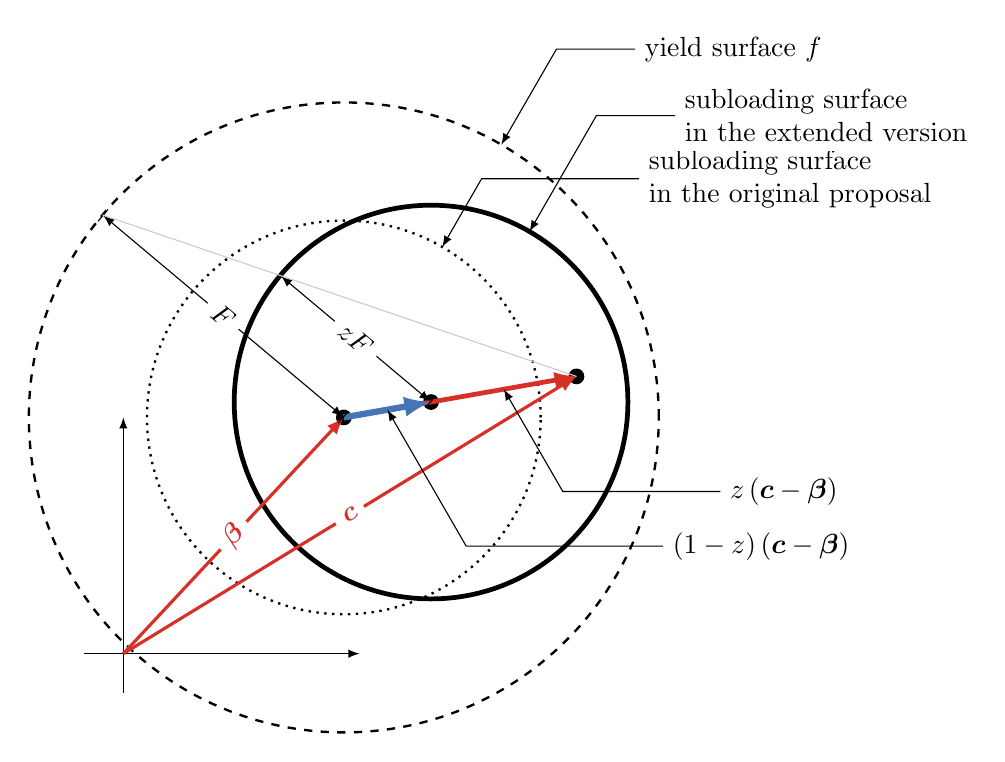
\begin{tikzpicture}[>=latex]
    \newcommand{\FF}{4}
    \newcommand{\SF}{2.5}
    \draw[->](-.5,0)--(3,0);
    \draw[->](0,-.5)--(0,3);
    \coordinate(A)at(2.8,3);
    \coordinate(B)at($(A)+(10:3)$);
    \coordinate(C)at($(B)!\SF/\FF!(A)$);
    \node[fill=black,circle,inner sep=0,minimum size=2mm]at(A){};
    \node[fill=black,circle,inner sep=0,minimum size=2mm]at(B){};
    \node[fill=black,circle,inner sep=0,minimum size=2mm]at(C){};
    \draw[dashed,draw,line width=.3mm](A)circle(\FF);
    \draw[dotted,draw,line width=.3mm](A)circle(\SF);
    \draw[draw,line width=.6mm](C)circle(\SF);
    \draw[->,d73027,line width=.4mm](0,0)--(A)node[midway,fill=white,sloped]{$\bbeta$};
    \draw[->,d73027,line width=.6mm](A)--(B);
    \draw[->,d73027,line width=.4mm](0,0)--(B)node[midway,fill=white,sloped]{$\bc$};
    \draw[->,4575b4,line width=.8mm](A)--(C);
    \draw[|<->|](A)--++(140:\FF)node[midway,fill=white,sloped]{$F$};
    \draw[|<->|](C)--++(140:\SF)node[midway,fill=white,sloped]{$zF$};
    \draw[<-]($(A)+(60:\FF)$)--++(60:1.4)--++(1,0)node[right,fill=white]{yield surface $f$};
    \draw[<-]($(A)+(60:\SF)$)--++(60:1)--++(2,0)node[right,fill=white,align=left]{subloading surface\\in the original proposal};
    \draw[<-]($(C)+(60:\SF)$)--++(60:1.7)--++(1,0)node[right,fill=white,align=left]{subloading surface\\in the extended version};
    \draw[<-]($(C)!.5!(B)$)--++(-60:1.5)--++(2,0)node[right,fill=white]{$z\left(\bc-\bbeta\right)$};
    \draw[<-]($(A)!.5!(C)$)--++(-60:2)--++(2.5,0)node[right,fill=white]{$\left(1-z\right)\left(\bc-\bbeta\right)$};
    \draw[black!20]($(A)+(140:\FF)$)--(B);
\end{tikzpicture}
\begin{tikzpicture}
    \begin{axis}[axis lines=middle,xlabel=$x$,ylabel=$y$,grid=both,width=6.5cm,height=4.5cm,legend pos=south east,ymin=0,ymax=1.5,scale only axis,enlargelimits=false]
        \pgfmathsetmacro{\aa}{-.05}
        \pgfmathsetmacro{\bb}{1}
        \addplot[line width=2pt,dashed,domain=0:10,samples=100,color=fc8d59]{\aa*x+\bb};
        \addplot[line width=1pt,domain=0:10,samples=100,color=d73027]{\aa*x+\bb+(\aa-\bb)*exp(-x)-\aa};
        \addplot[line width=1pt,color=4575b4] table [x index=0, y index=1, col sep=space] {tmp/softening.inverse.txt};
        \addlegendentry{$a(x)=\aa{}x+\bb$}
        \addlegendentry{$\dot{y}=a(x)-y$}
        \addlegendentry{$\dot{y}=1-y/a(x)$}
    \end{axis}
\end{tikzpicture}
\begin{tikzpicture}
    \begin{axis}[axis lines=middle,xlabel=$x$,ylabel=$y$,grid=both,width=6.5cm,height=4.5cm,legend pos=south east,ymin=0,ymax=1.5,scale only axis,enlargelimits=false]
        \pgfmathsetmacro{\aa}{0.05}
        \pgfmathsetmacro{\bb}{1}
        \addplot[line width=2pt,dashed,domain=0:10,samples=100,color=fc8d59]{\aa*x+\bb};
        \addplot[line width=1pt,domain=0:10,samples=100,color=d73027]{\aa*x+\bb+(\aa-\bb)*exp(-x)-\aa};
        \addplot[line width=1pt,color=4575b4] table [x index=0, y index=1, col sep=space] {tmp/hardening.inverse.txt};
        \addlegendentry{$a(x)=\aa{}x+\bb$}
        \addlegendentry{$\dot{y}=a(x)-y$}
        \addlegendentry{$\dot{y}=1-y/a(x)$}
    \end{axis}
\end{tikzpicture}
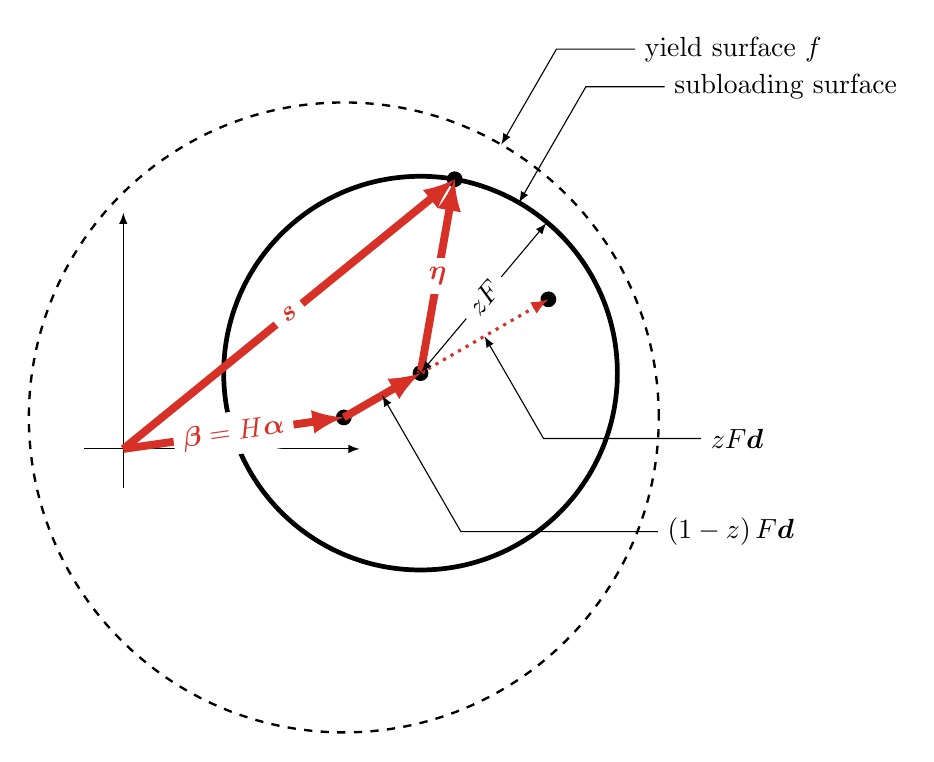
\begin{tikzpicture}[>=latex]
    \newcommand{\DD}{80}
    \newcommand{\FF}{4}
    \newcommand{\SF}{2.5}
    \draw[->](-.5,0)--(3,0);
    \draw[->](0,-.5)--(0,3);
    \coordinate(A)at(2.8,.4);
    \coordinate(B)at($(A)+(30:3)$);
    \coordinate(C)at($(B)!\SF/\FF!(A)$);
    \coordinate(D)at($(C)+(\DD:\SF)$);
    \node[fill=black,circle,inner sep=0,minimum size=2mm]at(A){};
    \node[fill=black,circle,inner sep=0,minimum size=2mm]at(B){};
    \node[fill=black,circle,inner sep=0,minimum size=2mm]at(C){};
    \node[fill=black,circle,inner sep=0,minimum size=2mm]at(D){};
    \draw[dashed,draw,line width=.3mm](A)circle(\FF);
    \draw[draw,line width=.6mm](C)circle(\SF);
    \draw[->,d73027,line width=1mm](0,0)--(A)node[midway,fill=white,sloped]{$\bbeta=H\balpha$};
    \draw[->,dotted,d73027,line width=.4mm](C)--(B);
    \draw[->,d73027,line width=1mm](A)--(C);
    \draw[->,d73027,line width=1mm](C)--(D)node[midway,fill=white]{$\beeta$};
    \draw[->,d73027,line width=1mm](0,0)--(D)node[midway,fill=white,sloped]{$\bs$};
    \draw[|<->|](C)--++(50:\SF)node[midway,fill=white,sloped]{$zF$};
    \draw[<-]($(A)+(60:\FF)$)--++(60:1.4)--++(1,0)node[right,fill=white]{yield surface $f$};
    \draw[<-]($(C)+(60:\SF)$)--++(60:1.7)--++(1,0)node[right,fill=white]{subloading surface};
    \draw[<-]($(C)!.5!(B)$)--++(-60:1.5)--++(2,0)node[right,fill=white]{$zF\bd$};
    \draw[<-]($(A)!.5!(C)$)--++(-60:2)--++(2.5,0)node[right,fill=white]{$\left(1-z\right)F\bd$};
\end{tikzpicture}
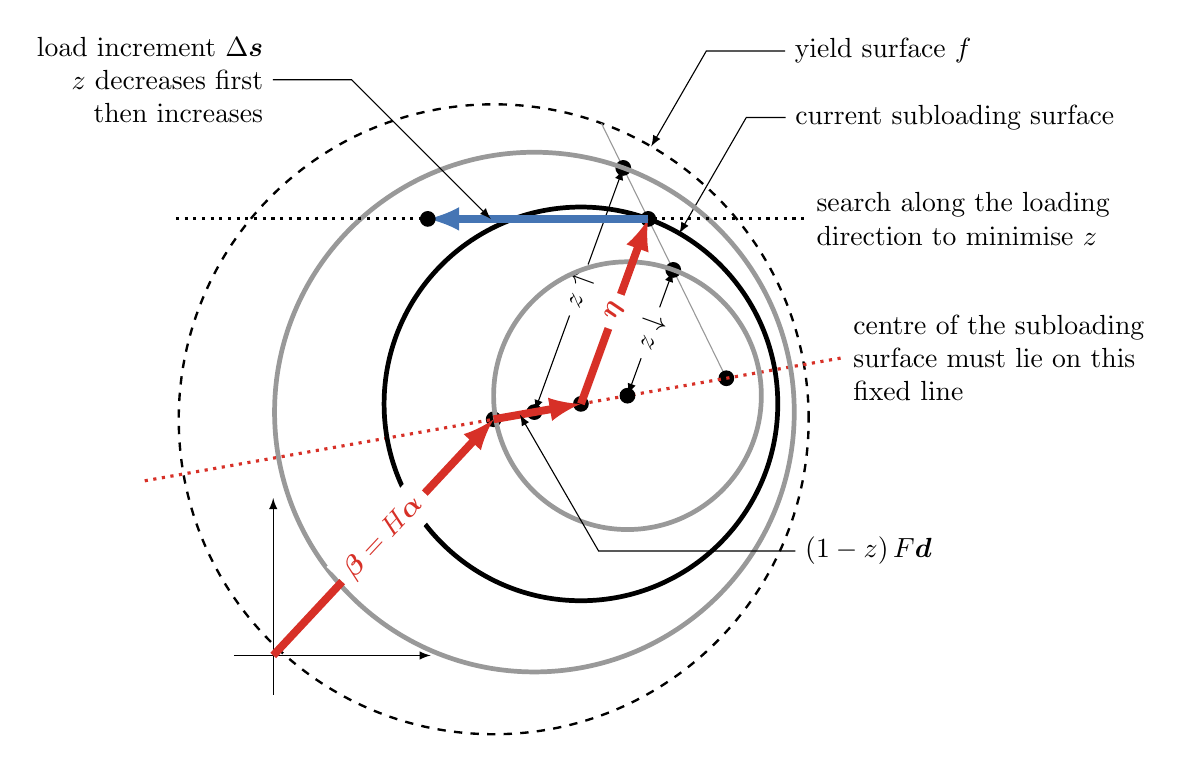
\begin{tikzpicture}[>=latex]
    \newcommand{\DD}{70}
    \newcommand{\FF}{4}
    \newcommand{\SF}{2.5}
    \newcommand{\BF}{3.3}
    \newcommand{\LF}{1.7}
    \draw[->](-.5,0)--(2,0);
    \draw[->](0,-.5)--(0,2);
    % yield surface
    \coordinate(A)at(2.8,3);
    \node[fill=black,circle,inner sep=0,minimum size=2mm]at(A){};
    \draw[dashed,draw,line width=.3mm](A)circle(\FF);
    \draw[<-]($(A)+(60:\FF)$)--++(60:1.4)--++(1,0)node[right,fill=white]{yield surface $f$};
    % similarity centre
    \coordinate(B)at($(A)+(10:3)$);
    \draw[black!40](B)--($(A)+(\DD:\FF)$);
    \node[fill=black,circle,inner sep=0,minimum size=2mm]at(B){};
    \draw[dotted,d73027,line width=.4mm]($(B)!2.5!(A)$)--($(A)!1.5!(B)$)node[black,right,align=left]{centre of the subloading\\surface must lie on this\\fixed line};
    % current subloading surface
    \coordinate(C)at($(B)!\SF/\FF!(A)$);
    \node[fill=black,circle,inner sep=0,minimum size=2mm]at(C){};
    \draw[draw,line width=.6mm](C)circle(\SF);
    \draw[<-]($(C)+(60:\SF)$)--++(60:1.7)--++(.5,0)node[right,fill=white]{current subloading surface};
    \coordinate(D)at($(C)+(\DD:\SF)$);
    \node[fill=black,circle,inner sep=0,minimum size=2mm]at(D){};
    % bigger subloading surface
    \coordinate(CB)at($(B)!\BF/\FF!(A)$);
    \node[fill=black,circle,inner sep=0,minimum size=2mm]at(CB){};
    \node[fill=black,circle,inner sep=0,minimum size=2mm]at($(CB)+(\DD:\BF)$){};
    \draw[|<->|](CB)--++(\DD:\BF)node[midway,fill=white,sloped]{$z\uparrow$};
    \draw[black!40,draw,line width=.6mm](CB)circle(\BF);
    % smaller subloading surface
    \coordinate(CS)at($(B)!\LF/\FF!(A)$);
    \node[fill=black,circle,inner sep=0,minimum size=2mm]at(CS){};
    \node[fill=black,circle,inner sep=0,minimum size=2mm]at($(CS)+(\DD:\LF)$){};
    \draw[|<->|](CS)--++(\DD:\LF)node[midway,fill=white,sloped]{$z\downarrow$};
    \draw[black!40,draw,line width=.6mm](CS)circle(\LF);
    % arrows
    \draw[->,d73027,line width=1mm](0,0)--(A)node[midway,fill=white,sloped]{$\bbeta=H\balpha$};
    \draw[->,d73027,line width=1mm](A)--(C);
    \draw[->,d73027,line width=1mm](C)--(D)node[midway,fill=white,sloped]{$\beeta$};
    \draw[<-]($(A)!0.3!(C)$)--++(-60:2)--++(2.5,0)node[right,fill=white]{$\left(1-z\right)F\bd$};
    \draw[dotted,line width=.4mm]($(D)+(180:6)$)--($(D)+(0:2)$)node[right,align=left]{search along the loading\\direction to minimise $z$};
    \draw[->,4575b4,line width=1mm](D)--++(180:2.8)node[fill=black,circle,inner sep=0,minimum size=2mm]{};
    \draw[<-]($(D)+(180:2)$)--++(135:2.5)--++(-1,0)node[left,align=right]{load increment $\Delta\bs$\\$z$ decreases first\\then increases};
\end{tikzpicture}
\begin{tikzpicture}
    \begin{axis}[
            xlabel={$z$},
            ylabel={$\text{rcond}\left(\mb{J}\right)$},
            legend pos=south east,
            grid=major,
            width=7cm,
            height=4.5cm,
            xmode=log,
            ymode=log,
            xmin=1e-16,
            xmax=1e-1,
            scale only axis,
            enlargelimits=false,
        ]
        \addplot[thick,mark=diamond*, color=d73027] table [x index=0, y index=1, col sep=space] {tmp/log.txt};
        \addlegendentry{$-\ln\left(z\right)$}
        \addplot[thick,mark=*, color=fc8d59] table [x index=0, y index=1, col sep=space] {tmp/pow3.txt};
        \addlegendentry{$z^{-0.2}$}
        \addplot[thick,mark=square*, color=fee090] table [x index=0, y index=1, col sep=space] {tmp/pow1.txt};
        \addlegendentry{$z^{-0.5}$}
        \addplot[thick,mark=triangle*, color=e0f3f8] table [x index=0, y index=1, col sep=space] {tmp/pow2.txt};
        \addlegendentry{$z^{-1}$}
        \addplot[thick,mark=o, color=91bfdb] table [x index=0, y index=1, col sep=space] {tmp/cot.txt};
        \addlegendentry{$\cot\left(z\right)$}
        \addplot[thick,mark=+, color=4575b4] table [x index=0, y index=1, col sep=space] {tmp/pow4.txt};
        \addlegendentry{$z^{-2}$}
    \end{axis}
\end{tikzpicture}
\begin{tikzpicture}[spy using outlines={circle,magnification=3,size=3cm,connect spies}]
    \begin{axis}[
            xlabel={analysis step time $t$},
            ylabel={normal yield ratio $z$},
            legend pos=north east,
            grid=major,
            width=6.5cm,
            height=4.5cm,
            xmin=0,
            xmax=2,
            ymax=.6,
            scale only axis,
            enlargelimits=false,
        ]
        \addplot[mark=x,color=d73027,line width=.5pt] table [x index=0, y index=3, col sep=space] {tmp/conventional.criterion.txt};
        \addlegendentry{conventional}
        \addplot[mark=+,color=4575b4,line width=.5pt] table [x index=0, y index=3, col sep=space] {tmp/new.criterion.txt};
        \addlegendentry{corrected}
        \spy[]on(4.1,.85)in node[fill=white]at(1.6,1.7);
    \end{axis}
\end{tikzpicture}
\begin{tikzpicture}[spy using outlines={circle,magnification=3,size=3cm,connect spies}]
    \begin{axis}[
            xlabel={analysis step time $t$},
            ylabel={accumulated plastic strain $q$},
            legend pos=south east,
            grid=major,
            width=6.5cm,
            height=4.5cm,
            xmin=0,
            xmax=2,
            scale only axis,
            enlargelimits=false,
        ]
        \addplot[mark=x,color=d73027,line width=.5pt] table [x index=0, y index=2, col sep=space] {tmp/conventional.criterion.txt};
        \addlegendentry{conventional}
        \addplot[mark=+,color=4575b4,line width=.5pt] table [x index=0, y index=2, col sep=space] {tmp/new.criterion.txt};
        \addlegendentry{corrected}
        \spy[]on(4,2.7)in node[fill=white]at(1.6,2.9);
    \end{axis}
\end{tikzpicture}
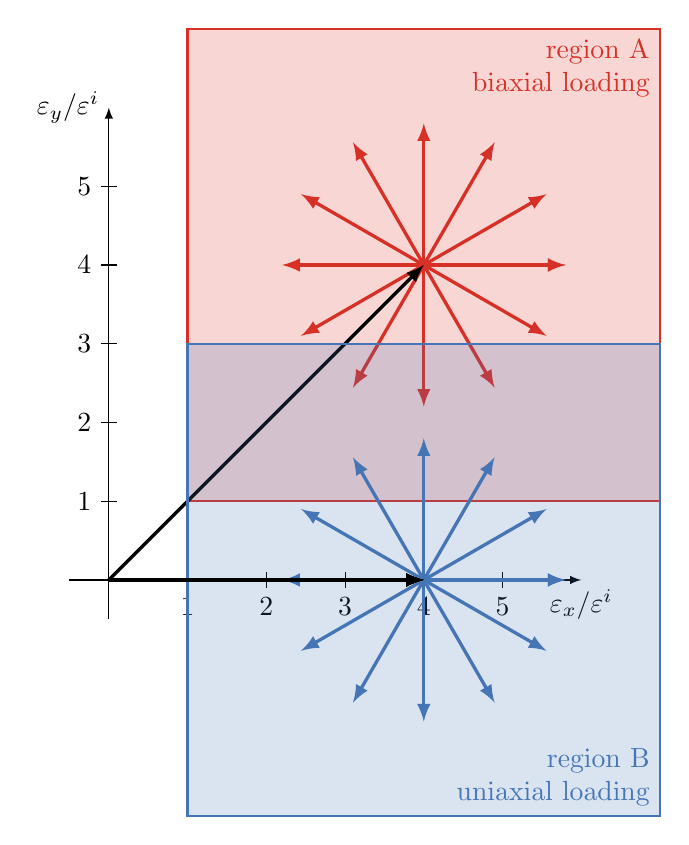
\begin{tikzpicture}[>=latex]
\draw[->](-.5,0)--(6,0)node[below]{$\varepsilon_x/\varepsilon^i$};
\draw[->](0,-.5)--(0,6)node[left]{$\varepsilon_y/\varepsilon^i$};
\foreach \i in {1,...,5} {
        \draw(\i,0.1)--(\i,-0.1)node[below]{\i};
        \draw(0.1,\i)--(-0.1,\i)node[left]{\i};
    }
\draw[thick,d73027,fill=d73027,fill opacity=.2,text opacity=1](1,1)rectangle++(6,6)node[anchor=north east,align=right]{region A\\biaxial loading};
\def\n{12}
\foreach \i in {0,...,\n} {
        \draw[->,very thick,d73027](4,4)--++(\i*360/\n:1.8);
    }
\draw[very thick,->](0,0)--(4,4);
\draw[thick,4575b4,fill=4575b4,fill opacity=.2,text opacity=1](1,3)rectangle++(6,-6)node[anchor=south east,align=right]{region B\\uniaxial loading};
\foreach \i in {0,...,\n} {
\draw[->,very thick,4575b4](4,0)--++(\i*360/\n:1.8);
\draw[very thick,->](0,0)--(4,0);
}
\end{tikzpicture}
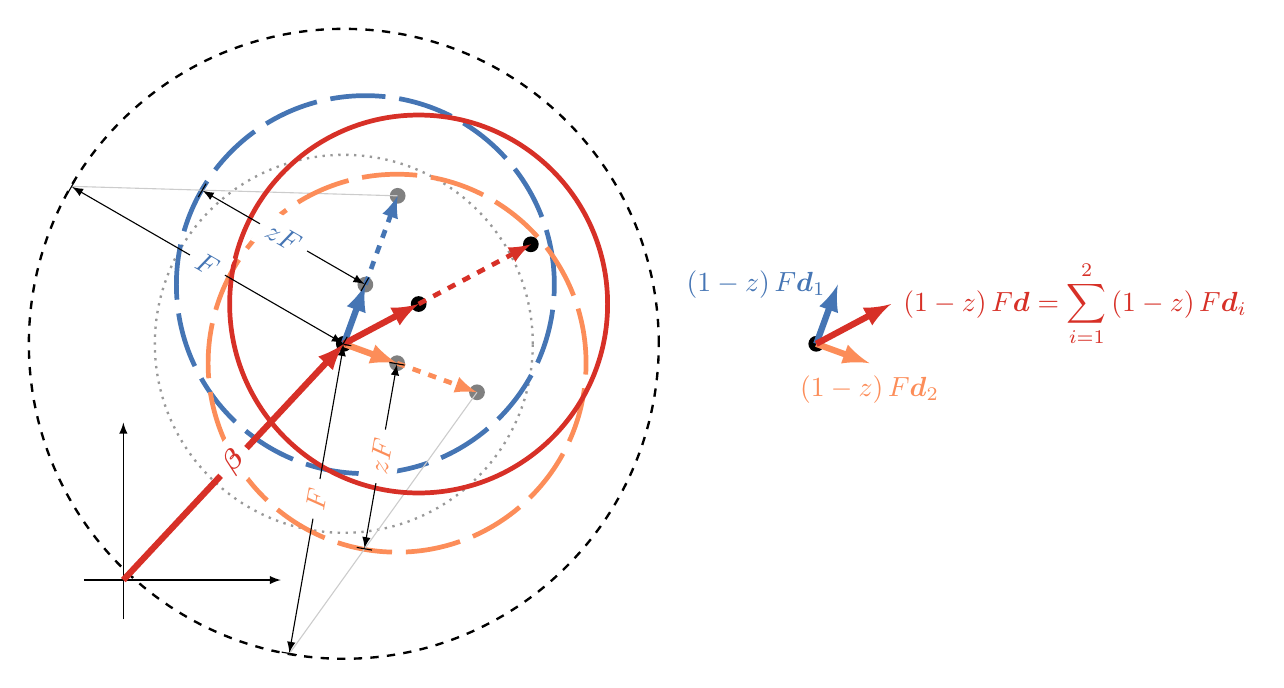
\begin{tikzpicture}[>=latex]
    \newcommand{\FF}{4}
    \newcommand{\SF}{2.4}
    \newcommand{\DD}{150}
    \draw[->](-.5,0)--(2,0);
    \draw[->](0,-.5)--(0,2);
    \coordinate(A)at(2.8,3);
    \coordinate(B)at($(A)+(70:2)$);
    \coordinate(C)at($(B)!\SF/\FF!(A)$);
    \node[fill=black,circle,inner sep=0,minimum size=2mm]at(A){};
    \node[fill=black!50,circle,inner sep=0,minimum size=2mm]at(B){};
    \node[fill=black!50,circle,inner sep=0,minimum size=2mm]at(C){};
    \draw[dashed,draw,line width=.3mm](A)circle(\FF);
    \draw[dotted,draw,black!40,line width=.3mm](A)circle(\SF);
    \draw[draw,dash pattern=on 20pt off 5pt,4575b4,line width=.6mm](C)circle(\SF);
    \draw[->,4575b4,dashed,line width=.6mm](C)--(B);
    \draw[->,4575b4,line width=.8mm](A)--(C);
    \draw[black!20]($(A)+(\DD:\FF)$)--(B);
    \newcommand{\DE}{-100}
    \coordinate(E)at($(A)+(-20:1.8)$);
    \coordinate(F)at($(E)!\SF/\FF!(A)$);
    \node[fill=black!50,circle,inner sep=0,minimum size=2mm]at(E){};
    \node[fill=black!50,circle,inner sep=0,minimum size=2mm]at(F){};
    \draw[draw,dash pattern=on 20pt off 5pt,fc8d59,line width=.6mm](F)circle(\SF);
    \draw[->,fc8d59,dashed,line width=.6mm](F)--(E);
    \draw[->,fc8d59,line width=.8mm](A)--(F);
    \draw[black!20]($(A)+(\DE:\FF)$)--(E);
    \coordinate(G)at($(F)+(C)-(A)$);
    \coordinate(H)at($(B)+(E)-(A)$);
    \node[fill=black,circle,inner sep=0,minimum size=2mm]at(G){};
    \node[fill=black,circle,inner sep=0,minimum size=2mm]at(H){};
    \draw[->,d73027,line width=.8mm](A)--(G);
    \draw[->,d73027,dashed,line width=.6mm](G)--(H);
    \draw[draw,d73027,line width=.6mm](G)circle(\SF);
    \draw[|<->|](A)--++(\DD:\FF)node[midway,4575b4,fill=white,sloped]{$F$};
    \draw[|<->|](C)--++(\DD:\SF)node[midway,4575b4,fill=white,sloped]{$zF$};
    \draw[|<->|](A)--++(\DE:\FF)node[midway,fc8d59,fill=white,sloped]{$F$};
    \draw[|<->|](F)--++(\DE:\SF)node[midway,fc8d59,fill=white,sloped]{$zF$};
    \draw[->,d73027,line width=.8mm](0,0)--(A)node[midway,fill=white,sloped]{$\bbeta$};
    \begin{scope}
        \node[fill=black,circle,inner sep=0,minimum size=2mm]at($(A)+(6,0)$){};
        \draw[->,4575b4,line width=.8mm]($(A)+(6,0)$)--($(C)+(6,0)$)node[left]{$\left(1-z\right)F\bd_1$};
        \draw[->,fc8d59,line width=.8mm]($(A)+(6,0)$)--($(F)+(6,0)$)node[below]{$\left(1-z\right)F\bd_2$};
        \draw[->,d73027,line width=.8mm]($(A)+(6,0)$)--($(G)+(6,0)$)node[right]{$\displaystyle\left(1-z\right)F\bd=\sum^{2}_{i=1}\left(1-z\right)F\bd_i$};
    \end{scope}
\end{tikzpicture}
\end{document}